\documentclass[border=10pt]{standalone}
\usepackage{tikz}\usepackage{amsmath}\usetikzlibrary{arrows.meta}
\begin{document}
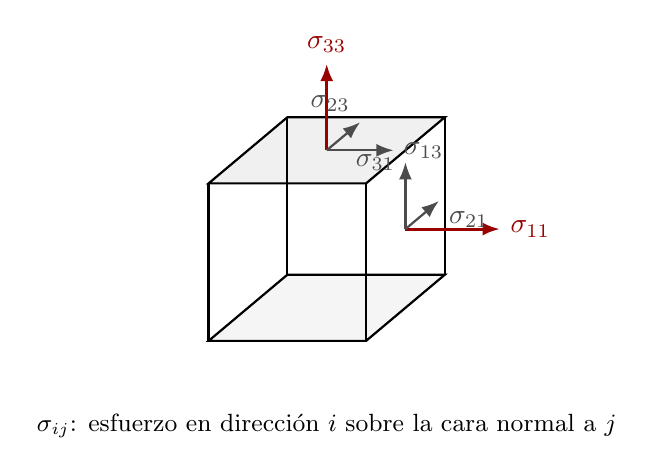
\begin{tikzpicture}[x={(1cm,0cm)},y={(0.5cm,0.42cm)},z={(0cm,1cm)},line width=0.8pt,>={Latex[length=2.2mm]}]
  \draw[fill=black!4] (0,0,0)--(2,0,0)--(2,2,0)--(0,2,0)--cycle;
  \draw[fill=black!6] (0,0,2)--(2,0,2)--(2,2,2)--(0,2,2)--cycle;
  \draw (0,0,0)--(0,0,2) (2,0,0)--(2,0,2) (2,2,0)--(2,2,2) (0,2,0)--(0,2,2);
  % cara +x1 (frente): normal sigma_11, cortantes sigma_21, sigma_31
  \draw[->,red!60!black,line width=1.1pt] (2,1,1)--++(1.2,0,0) node[right]{$\sigma_{11}$};
  \draw[->,black!70] (2,1,1)--++(0,0,0.85) node[left]{$\sigma_{31}$};
  \draw[->,black!70] (2,1,1)--++(0,0.85,0) node[below right]{$\sigma_{21}$};
  % cara +x3 (top): normal sigma_33, cortantes sigma_13, sigma_23
  \draw[->,red!60!black,line width=1.1pt] (1,1,2)--++(0,0,1.1) node[above]{$\sigma_{33}$};
  \draw[->,black!70] (1,1,2)--++(0.85,0,0) node[right]{$\sigma_{13}$};
  \draw[->,black!70] (1,1,2)--++(0,0.85,0) node[above left]{$\sigma_{23}$};
  \node at (1,1,-1.5){\small $\sigma_{ij}$: esfuerzo en dirección $i$ sobre la cara normal a $j$};
\end{tikzpicture}
\end{document}
